%%%%
% Additional packages to support the book, not part of the APEX style.
%%%%
\usepackage{fancyhdr}
\usepackage{eso-pic}
\usepackage{lipsum}
%\usepackage{pgfplots}
%\pgfplotsset{width=\marginparwidth+1pt,compat=1.3}
\usepackage[font=small]{caption}
%,justification=centering

%%%%
%% These are low level LaTeX commands that determine the 
%% look of the Chapter and Section headings.
%% Note the use in the chapter part of an external file
%% that contains graphics for each chapter start.
%%%%

%%%%
%% Commands for the header, utilizing the fancyhdr
%% (fancy header) package
%%%%

\pagestyle{fancy}
\fancyhead{}
\fancyfoot{}
\renewcommand{\chaptermark}[1]{\markboth{\chaptername\ \thechapter\ \ \ \ {#1}}{}}
\renewcommand{\sectionmark}[1]{\markright{\thesection\ \ \ \  #1}}
\fancyhf{}         %Clears all header and footer fields, in preparation.
\renewcommand{\headrulewidth}{0pt}
\renewcommand{\footrulewidth}{0pt}

\ifthenelse{\boolean{longpage}}%
{}% end header of longpage
{% begin header/footer of not longpage
\fancyhfoffset[LE,RO]{\marginparwidth+\marginparsep}
%\fancyfoot[LE,RO]{\textbf{\thepage}} %Displays the page number in bold in the header,

\fancyfoot[LE]{\begin{minipage}{\textwidth}%
\noindent\hskip\marginparwidth\hskip\marginparsep\hskip-4pt\rule{\textwidth}{.4pt}
\vskip.2\baselineskip
\noindent\hskip\marginparwidth\hskip\marginparsep\hskip-4pt%
Notes:
\vskip 1.5in\textbf{\thepage}
\end{minipage}} 

\fancyfoot[RO]{\begin{minipage}{\textwidth+\marginparwidth+\marginparsep}%
\rule{\textwidth-\marginparwidth-\marginparsep}{.4pt}
\vskip.2\baselineskip
Notes:
\vskip 1.5in
\hfill\textbf{\thepage}
\end{minipage}}       


\fancyhead[LE]{\nouppercase{\leftmark}}
      %Displays the upper-level (chapter) information---
      % as determined above---in non-upper case in the header, 
      %to the right on even pages.
\fancyhead[RO]{\rightmark}
			%Displays the lower-level (section) information---as
      % determined above---in the header, to the left on odd pages.
      
}% End the ifthenelse{longpage}


\ifthenelse{\boolean{longpage}}% for changing the header
{% longpage
\newcommand{\exerciseheader}{}
\newcommand{\regularheader}{}
\newcommand{\endmatheader}{}
}% i.e, the above does nothing
{% now for a real change
\newcommand{\exerciseheader}{%
				\fancyhfoffset[LE,RO]{32pt}%
				\fancyfoot[LE]{\textbf{\thepage}}% 
				\fancyfoot[RO]{\textbf{\thepage}}
				\fancyhead{}% 
}

\newcommand{\regularheader}{%
\fancyhead[LE]{\nouppercase{\leftmark}}%
\fancyhead[RO]{\rightmark}%
\fancyfoot[LE]{\begin{minipage}{\textwidth}%
\noindent\hskip\marginparwidth\hskip\marginparsep\hskip0pt\rule{\textwidth}{.4pt}
\vskip.2\baselineskip
\noindent\hskip\marginparwidth\hskip\marginparsep\hskip0pt%
Notes:
\vskip 1.5in\textbf{\thepage}
\end{minipage}} 

\fancyfoot[RO]{\begin{minipage}{\textwidth+\marginparwidth+\marginparsep}%
\rule{\textwidth-\marginparwidth-\marginparsep}{.4pt}
\vskip.2\baselineskip
Notes:
\vskip 1.5in
\hfill\textbf{\thepage}
\end{minipage}}
\fancyhfoffset[LE,RO]{\marginparsep+\marginparwidth}
}

\newcommand{\qendheader}{%
		\fancyhead{}%
		\fancyfoot{}%
		}
}% ends if/then/else exercise/regular headers


%
%  Defining what the chapter titles look like
%

\newdimen\titleheight

\makeatletter
\def\@makechapterhead#1{%
  {\parindent \z@ \raggedright \reset@font
    {\Huge \thechapter: \parbox[t]{.85\linewidth}{\parindent \z@ \raggedright \reset@font\scshape \textsc #1}}
    \par\vskip 10\p@
    \hrule height 1pt
    \vskip 10\p@
  }}
%chapter title of V3.0

%\makeatletter
%\def\@makechapterhead#1{%
  %{\parindent \z@ \raggedright \reset@font
    %{\Huge \thechapter: \scshape \textsc #1}
    %\par\vskip 10\p@
    %\hrule height 1pt
    %\vskip 10\p@
  %}}	
%%
%% ends chapter title of V3.0
	
%%  
%%%\makeatletter
%%\def\@makesectionhead#1{%
%%	 {\reset@font\LARGE\itshape\bfseries\strut #1 \thechapter.\thesection \ #1
%%	 }}

%%%%
%%
%%  For figures in the margin
%%
%%%%

%%\usepackage{wrapfig}
%%
%%\setlength{\marginparsep}{10pt}
%%\setlength{\wrapoverhang}{\marginparwidth}
%%\addtolength{\wrapoverhang}{\marginparsep}
%%
%%%\newenvironment{mfigure}[1]{%
%%%    \wrapfigure{#1}{0pt}%
%%%    \begin{minipage}{\marginparwidth}%
%%%    \centering%
%%%}{%
%%%    \end{minipage}%
%%%    \endwrapfigure%
%%%}

\counterwithin{figure}{section}

\ifthenelse{\boolean{longpage}}%
		{\newcommand{\mfigure}[5][]{%
		\vskip \baselineskip%
			\noindent\begin{minipage}{\textwidth}
  			\centering
  			\myincludegraphics{#5}
  			#1%
  			\captionsetup{type=figure}
	  		\caption{#3}\label{#4}
  		\end{minipage}
		}}
		{\newcommand{\mfigure}[5][]{%
		\ifthenelse{\isodd{\thepage}}%
			{\AddToShipoutPicture*{\put(427,\LenToUnit{#2\paperheight}){%
			\begin{minipage}{\marginparwidth}%
				\centering%
	  		\myincludegraphics[#1]{#5}%
  			\captionsetup{type=figure}%
  			%#1%
	  		\caption{#3}\label{#4}%
  		\end{minipage}}}}%
			{\AddToShipoutPicture*{\put(36,\LenToUnit{#2\paperheight}){%
			\begin{minipage}{\marginparwidth}%
			  \centering%
  		  \myincludegraphics[#1]{#5}%
  			\captionsetup{type=figure}%
  			%#1%
	  		\caption{#3}\label{#4}%
  		\end{minipage}}}}%
		}}%

\ifthenelse{\boolean{longpage}}%
		{\newcommand{\mtable}[4]{
					\vskip \baselineskip%
					\noindent\begin{minipage}{\textwidth}
  					\centering\small
  					#4
  					\captionsetup{type=figure}
	  				\caption{#2}\label{#3}
  				\end{minipage}
  				\vskip\baselineskip}
  	}
		{\newcommand{\mtable}[4]{%
			\ifthenelse{\isodd{\thepage}}%
				{\AddToShipoutPicture*{\put(427,\LenToUnit{#1\paperheight}){%
					\begin{minipage}{\marginparwidth}%
  					\centering\small%
  					#4%
  					\captionsetup{type=figure}%
	  				\caption{#2}\label{#3}%
  				\end{minipage}}}}%
				{\AddToShipoutPicture*{\put(36,\LenToUnit{#1\paperheight}){%
					\begin{minipage}{\marginparwidth}%
 						 \centering\small%
 						 #4%
						  \captionsetup{type=figure}%
	  					\caption{#2}\label{#3}%
 					 \end{minipage}}}}%
		}}%

\ifthenelse{\boolean{longpage}}%
		{\newcommand{\mnote}[2]{%
					\hskip 25pt%
					\begin{minipage}{250pt}%
					\small%
					#2%
					\end{minipage}%
					\vskip\baselineskip%
		}%
		}%
		{\newcommand{\mnote}[2]{%
			\ifthenelse{\isodd{\thepage}}%
				{\AddToShipoutPicture*{\put(427,\LenToUnit{#1\paperheight}){%
					\begin{minipage}{\marginparwidth}
  					\small
  					#2
  				\end{minipage}}}}%
				{\AddToShipoutPicture*{\put(36,\LenToUnit{#1\paperheight}){%
					\begin{minipage}{\marginparwidth}
 						 \small
 						 #2
					\end{minipage}}}}
		}}


\newcommand{\showheightguidelines}{%
\AddToShipoutPicture{\put(10,\LenToUnit{.1\paperheight}){\tiny 10\%\rule{10pt}{1pt}}}
\AddToShipoutPicture{\put(10,\LenToUnit{.2\paperheight}){\tiny 20\%\rule{10pt}{1pt}}}
\AddToShipoutPicture{\put(10,\LenToUnit{.3\paperheight}){\tiny 30\%\rule{10pt}{1pt}}}
\AddToShipoutPicture{\put(10,\LenToUnit{.4\paperheight}){\tiny 40\%\rule{10pt}{1pt}}}
\AddToShipoutPicture{\put(10,\LenToUnit{.5\paperheight}){\tiny 50\%\rule{10pt}{1pt}}}
\AddToShipoutPicture{\put(10,\LenToUnit{.6\paperheight}){\tiny 60\%\rule{10pt}{1pt}}}
\AddToShipoutPicture{\put(10,\LenToUnit{.7\paperheight}){\tiny 70\%\rule{10pt}{1pt}}}
\AddToShipoutPicture{\put(10,\LenToUnit{.8\paperheight}){\tiny 80\%\rule{10pt}{1pt}}}
\AddToShipoutPicture{\put(10,\LenToUnit{.9\paperheight}){\tiny 90\%\rule{10pt}{1pt}}}
\AddToShipoutPicture{\put(580,\LenToUnit{.1\paperheight}){\rule{10pt}{1pt}\tiny 10\%}}
\AddToShipoutPicture{\put(580,\LenToUnit{.2\paperheight}){\rule{10pt}{1pt}\tiny 20\%}}
\AddToShipoutPicture{\put(580,\LenToUnit{.3\paperheight}){\rule{10pt}{1pt}\tiny 30\%}}
\AddToShipoutPicture{\put(580,\LenToUnit{.4\paperheight}){\rule{10pt}{1pt}\tiny 40\%}}
\AddToShipoutPicture{\put(580,\LenToUnit{.5\paperheight}){\rule{10pt}{1pt}\tiny 50\%}}
\AddToShipoutPicture{\put(580,\LenToUnit{.6\paperheight}){\rule{10pt}{1pt}\tiny 60\%}}
\AddToShipoutPicture{\put(580,\LenToUnit{.7\paperheight}){\rule{10pt}{1pt}\tiny 70\%}}
\AddToShipoutPicture{\put(580,\LenToUnit{.8\paperheight}){\rule{10pt}{1pt}\tiny 80\%}}
\AddToShipoutPicture{\put(580,\LenToUnit{.9\paperheight}){\rule{10pt}{1pt}\tiny 90\%}}
}

%\ifthenelse{\boolean{longpage}}%
		%{}
		%{\newcommand{\mfigurethree}[5][]{%
		%\ifthenelse{\isodd{\thepage}}%
			%{\AddToShipoutPicture*{\put(427,\LenToUnit{#2\paperheight}){%
			%\begin{minipage}{\marginparwidth}%
				%\centering%
	  		%\includemedia[#1]{\includegraphics{#5}}{#5.prc}%
  			%\captionsetup{type=figure}%
  			%%#1%
	  		%\caption{#3}\label{#4}%
  		%\end{minipage}}}}%
			%{\AddToShipoutPicture*{\put(36,\LenToUnit{#2\paperheight}){%
			%\begin{minipage}{\marginparwidth}%
			  %\centering%
  			%\includemedia[#1]{\includegraphics{#5}}{#5.prc}%
  			%\captionsetup{type=figure}%
  			%%#1%
	  		%\caption{#3}\label{#4}%
  		%\end{minipage}}}}%
		%}}%
		
		\newcommand{\mfigurethree}[6]{%
		\ifthenelse{\isodd{\thepage}}%
			{\AddToShipoutPicture*{\put(427,\LenToUnit{#3\paperheight}){%
			\begin{minipage}{\marginparwidth}%
				\centering%
				\ifthenelse{\boolean{in_threeD}}{% in 3D
	  		\includemedia[#1]{\includegraphics[#2]{#6_3D\colornamesuffix}}{#6_3D.prc}}%now not in 3D
				%{\includegraphics[width=150pt]{#6_3D\colornamesuffix}}%
				{\myincludegraphics[#2]{#6_3D}}%
  			\captionsetup{type=figure}%
  			%#1%
	  		\caption{#4}\label{#5}%
  		\end{minipage}}}}%
			{\AddToShipoutPicture*{\put(36,\LenToUnit{#3\paperheight}){%
			\begin{minipage}{\marginparwidth}%
			  \centering%
  			\ifthenelse{\boolean{in_threeD}}{% in 3D
	  		\includemedia[#1]{\includegraphics[#2]{#6_3D\colornamesuffix}}{#6_3D.prc}}%now not in 3D
				%{\includegraphics[width=150pt]{#6_3D\colornamesuffix}}%
				{\myincludegraphics[#2]{#6_3D}}%
  			\captionsetup{type=figure}%
  			%#1%
	  		\caption{#4}\label{#5}%
  		\end{minipage}}}}%
		}

%\AddToShipoutPicture{\ifthenelse{\ifodd{\thepage}}%
%{\put(10,10){\begin{tikzpicture}\draw (0,0) circle (5pt);\end{tikzpicture}}}%
%{\put(100,100){\begin{tikzpicture}\draw (0,0) circle (5pt);\end{tikzpicture}}}}%
%

%\AddToShipoutPictureBG{%
% \AtPageLowerLeft{\hspace{1cm}A small logo: \rule{2cm}{3cm}}}
% 
%}{\AddToShipoutPicture*{\put(36,\LenToUnit{#2\paperheight})}}%
%{%
%\begin{minipage}{\marginparwidth}
%  \centering
%  \includegraphics{#1}
%  \captionof{figure}{#3}
%  \end{minipage}}}
%\AddToShipoutPicture*{\put(\LenToUnit{.5\paperwidth},\LenToUnit{.75\paperheight}){%
%  \begin{minipage}{100pt}
%  \centering
%  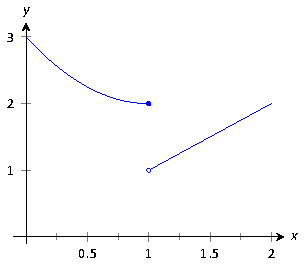
\includegraphics{test-figure2.pdf}
%  \captionof{figure}{Test caption}
%  \end{minipage}}}


%\newenvironment{mfigurefile}[2]{%
%\begin{tikzpicture}[remember picture,overlay]%
%\ifthenelse{\isodd{\thepage}}{\node [xshift=-36pt-.5\marginparwidth,yshift=#2\paperheight] at (current page.south east) }{\node [xshift=36pt+.5\marginparwidth,yshift=#2\paperheight] at (current page.south west) }%
%{\input{#1}};}%
%{\end{tikzpicture}%
%}

%\DeclareCaptionType{mytype}[Typename][List of mytype]


    
%%%%
%% End margin figure 
%%%%    
    

\newcommand{\bmx}[1]{\left[\hskip -3pt\begin{array}{#1} }
\newcommand{\emx}{\end{array}\hskip -3pt\right]}

\newcommand{\btz}{\begin{center}\begin{tikzpicture}}
\newcommand{\etz}{\end{tikzpicture}\end{center}}

\newcommand{\ds}{\displaystyle}

\newcommand{\fp}{\ensuremath{f\,'}}
\newcommand{\fpp}{\ensuremath{f\,''}}

\newcommand{\Fp}{\ensuremath{F\primeskip'}}
\newcommand{\Fpp}{\ensuremath{F\primeskip''}}

\newcommand{\yp}{\ensuremath{y\primeskip'}}
\newcommand{\gp}{\ensuremath{g\primeskip'}}

\newcommand{\dx}{\ensuremath{\Delta x}}
\newcommand{\dy}{\ensuremath{\Delta y}}
%\newcommand{\dz}{\ensuremath{\Delta z}}
\newcommand{\ddz}{\ensuremath{\Delta z}}

\newcommand{\thet}{\ensuremath{\theta}}
\newcommand{\norm}[1]{\ensuremath{||\ #1\ ||}}
\newcommand{\vnorm}[1]{\ensuremath{\norm{\vec #1}}}
\newcommand{\snorm}[1]{\ensuremath{\left|\left|\ #1\ \right|\right|}}
\newcommand{\la}{\left\langle}
\newcommand{\ra}{\right\rangle}
\newcommand{\dotp}[2]{\ensuremath{\vec #1 \cdot \vec #2}}
\newcommand{\proj}[2]{\ensuremath{\text{proj}_{\,\vec #2}{\,\vec #1}}}
\newcommand{\crossp}[2]{\ensuremath{\vec #1 \times \vec #2}}
\newcommand{\veci}{\ensuremath{\vec i}}
\newcommand{\vecj}{\ensuremath{\vec j}}
\newcommand{\veck}{\ensuremath{\vec k}}
\newcommand{\vecu}{\ensuremath{\vec u}}
\newcommand{\vecv}{\ensuremath{\vec v}}
\newcommand{\vecw}{\ensuremath{\vec w}}
\newcommand{\vecx}{\ensuremath{\vec x}}
\newcommand{\vecy}{\ensuremath{\vec y}}
\newcommand{\vrp}{\ensuremath{\vec r\, '}}
\newcommand{\vsp}{\ensuremath{\vec s\, '}}
\newcommand{\vrt}{\ensuremath{\vec r(t)}}
\newcommand{\vst}{\ensuremath{\vec s(t)}}
\newcommand{\vvt}{\ensuremath{\vec v(t)}}
\newcommand{\vat}{\ensuremath{\vec a(t)}}
\newcommand{\px}{\ensuremath{\partial x}}
\newcommand{\py}{\ensuremath{\partial y}}
\newcommand{\pz}{\ensuremath{\partial z}}
\newcommand{\pf}{\ensuremath{\partial f}}
\newcommand{\underlinespace}{\underline{\phantom{xxxxxx}}}

\newcommand{\surfaceS}{\ensuremath{\mathcal{S}}}

\newcommand{\mathN}{\ensuremath{\mathbb{N}}}

\newcommand{\zerooverzero}{\ensuremath{\ds \raisebox{8pt}{\text{``\ }}\frac{0}{0}\raisebox{8pt}{\text{\ ''}}}}


\newcommand{\myrule}{\rule[-4pt]{0pt}{13pt}}
\newcommand{\mmrule}{\rule[-10pt]{0pt}{15pt}}
\newcommand{\myds}{\ds\mmrule}
\newcommand{\deriv}[2]{\ensuremath{\myds\frac{d}{dx}\left(#1\right)=#2}}
\newcommand{\myint}[2]{\ensuremath{\myds\int #1\ dx=} \ensuremath{\ds #2}}

\DeclareMathOperator{\sech}{sech}
\DeclareMathOperator{\csch}{csch}
\DeclareMathOperator{\curl}{curl}
\DeclareMathOperator{\divv}{div}

\newcommand{\sword}[1]{\textbf{#1}}

\newcommand{\primeskip}{\hskip.75pt}

%%%% Begin Header TikZ

%  Some TiKZ  shortcuts to help make drawing 3D vectors faster.
%

\newcommand{\plotlinecolor}{blue}

%
% Draw x and y tick marks
%
\newcommand{\drawxticks}[1]
{\foreach \x in {#1}
		{\draw  (\x,-.1)--(\x,.1);
			};
}
\newcommand{\drawyticks}[1]
{\foreach \x in {#1}
		{\draw  (-.1,\x)--(.1,\x);
			};
}

\newcommand{\drawxlines}[3]
{\draw[<->] (#1,0) -- (#2,0) node [right] {$x$};
\foreach \x in {#3}
		{\draw  (\x,-.1)--(\x,.1);
			};
}

\newcommand{\drawylines}[3]
{\draw[<->] (0,#1) -- (0,#2) node [above] {$y$};
\foreach \x in {#3}
		{\draw  (-.1,\x)--(.1,\x);
			};
}

\newcommand{\drawxlabels}[1]
{\foreach \x in {#1}
		{\draw  (\x,-.1) node [below] {\scriptsize $\x$};
		};
}

\newcommand{\drawylabels}[1]
{\foreach \x in {#1}
		{\draw  (-.1,\x) node [left] {\scriptsize $\x$};
		};
}

%% draw a box of margin width size to see if figure is properly contained within
\newcommand{\marginsizebox}{\draw (0,0)--(\marginparwidth,0)--(\marginparwidth,3)--(0,3)--cycle;}

%%%%
%%%%

\newcommand{\asyouread}[1]{\begin{tikzpicture}
\ifthenelse{\boolean{in_color}}{\node [preaction={fill=black,opacity=.5,transform canvas={xshift=1mm,yshift=-1mm}}, right color=blue!80!black!30, left color=blue!80] at (0,0) {\textcolor{white}{\textsf{\textit{AS YOU READ $\ldots$}}}};}
{\node [preaction={fill=black,opacity=.5,transform canvas={xshift=1mm,yshift=-1mm}}, right color=black!30, left color=black!10] at (0,0) {\textcolor{white}{\textsf{\textit{AS YOU READ $\ldots$}}}};}
\end{tikzpicture}
\begin{enumerate}
#1
\end{enumerate}
\vskip 20pt}

%%%%
%%  A new figure environment, trying to fix the float problem.
%%
%%%%

%\newcounter{myfigurecounter}[chapter]
%\renewcommand\themyfigurecounter{\thechapter.\arabic{myfigurecounter}}
%\newenvironment{myfigure}{\refstepcounter{myfigurecounter}}{}
%\newcommand{\mycaption}[1]{%
%\begin{center}%
%\vskip -1.5\baselineskip
%\begin{tikzpicture}%
%\draw (0,0) node [text width=\textwidth,align=center] {Figure \themyfigurecounter: #1};%
%\end{tikzpicture}%
%\end{center}%
%}